\section{Studies of signal and background separation in cluster}
In the Future detector ,when energy of collision is upper, pileup is bigger and bigger, and the most important thing is that can separate signal and background efficiently. In this section, we want to study in different variables and see wether those can efficiently separate the signal and background in different detector size in cluster.\\

In the Figure 3 to 5, there are three variables about $c2b1$ , $\tau_{21}$, and $\tau_{32}$ signal efficiency versus background rejection rate plots. The criteria of separation efficiency is that, if the point is higher, it means it can separate the signal and background more efficiently.  Because at the same signal efficiency of different detector size, higher point means lower background efficiency, and that means it can separate well, and it will have the higher separation efficiency\\

We can see  $c2b1$ is the best way to separation, but the detector size can't improve the separation efficiency very well.$\tau_{21}$ can't improve the separation in different detector size at 10,20,40TeV, and $\tau_{32}$ has the good pattern to follow that the smaller detector size, the better the separation efficiency.In summary, $c2b1$ and $\tau_{32}$ are two variables that can suit for the higher energy for the future analysis.\\
\label{sec:efficiency}


\begin{figure}
\begin{center}
   \subfigure[5 TeV] {
   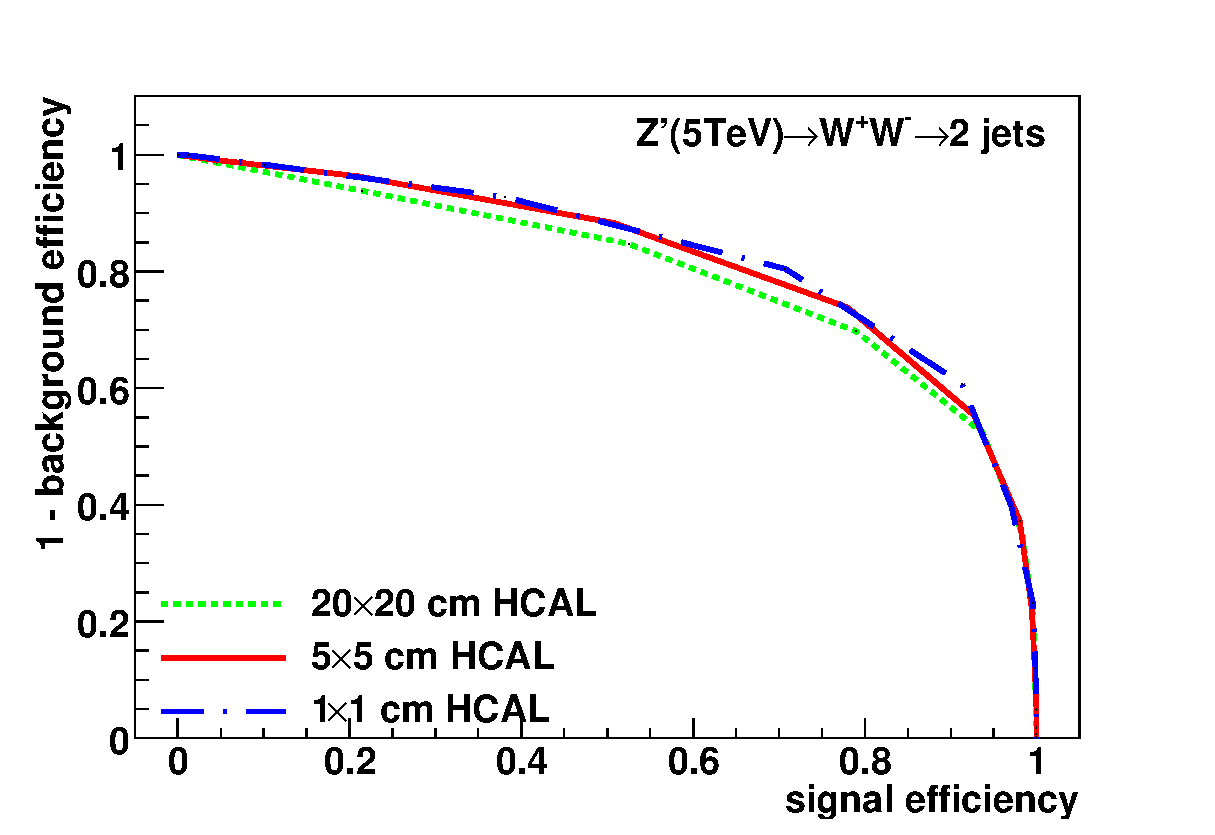
\includegraphics[width=0.43\textwidth]{figs/cluster_c2b1_5_tev_eff.eps}\hfill
   }
   \subfigure[10 TeV] {
   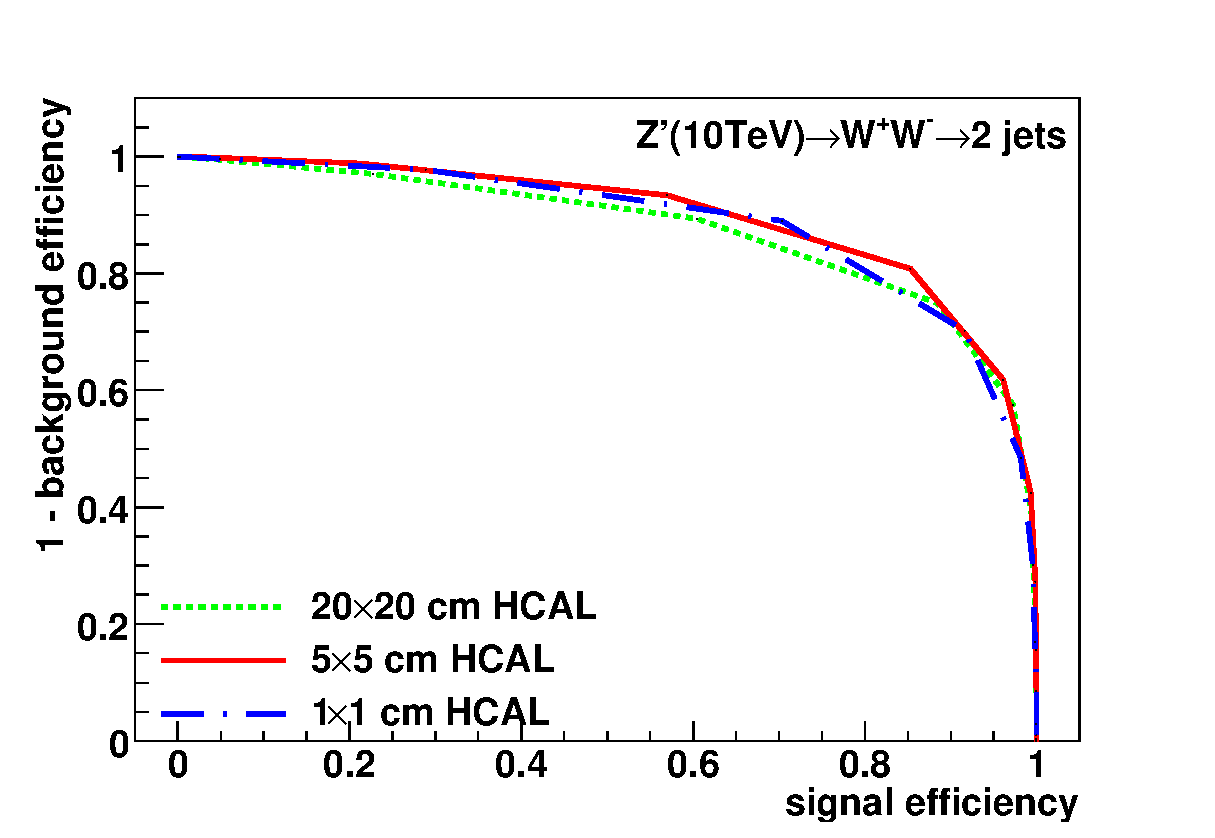
\includegraphics[width=0.43\textwidth]{figs/cluster_c2b1_10_tev_eff.eps}
   }
   \subfigure[20 TeV] {
   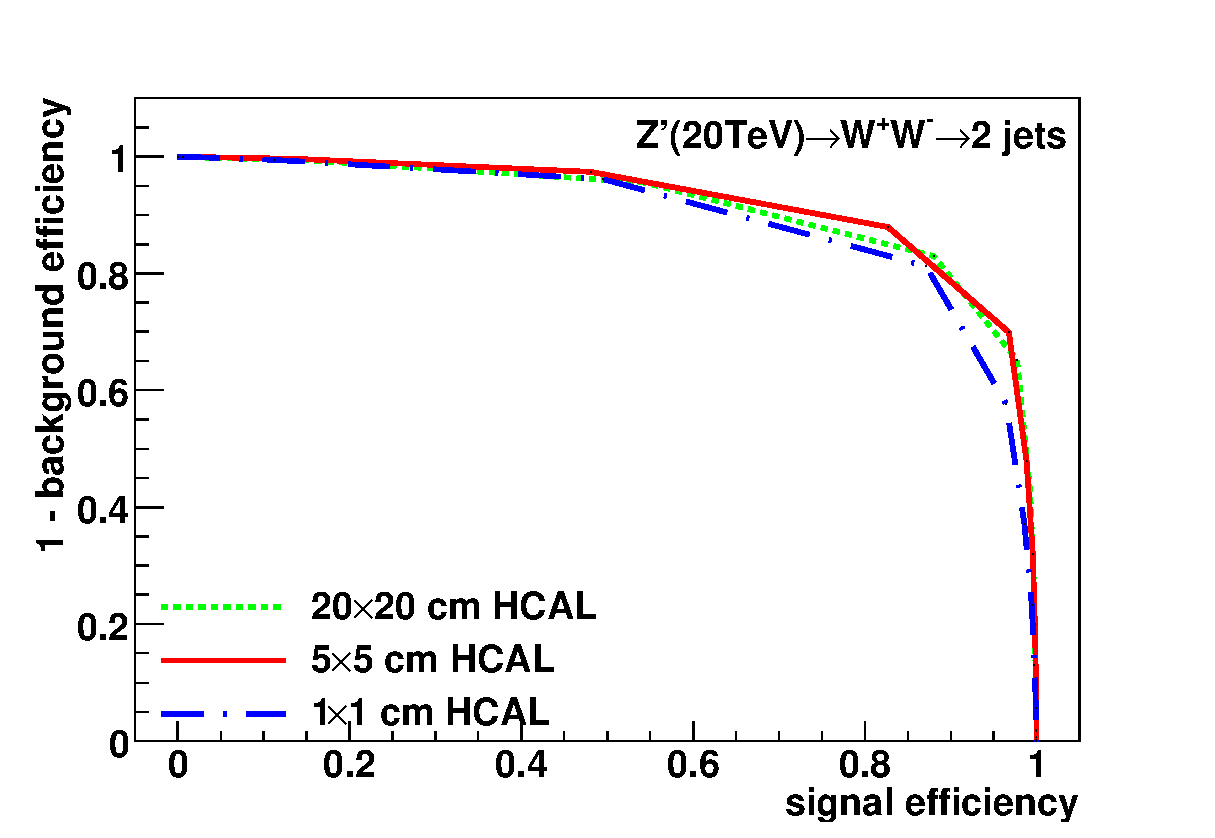
\includegraphics[width=0.43\textwidth]{figs/cluster_c2b1_20_tev_eff.eps}
   }
   \subfigure[40 TeV] {
   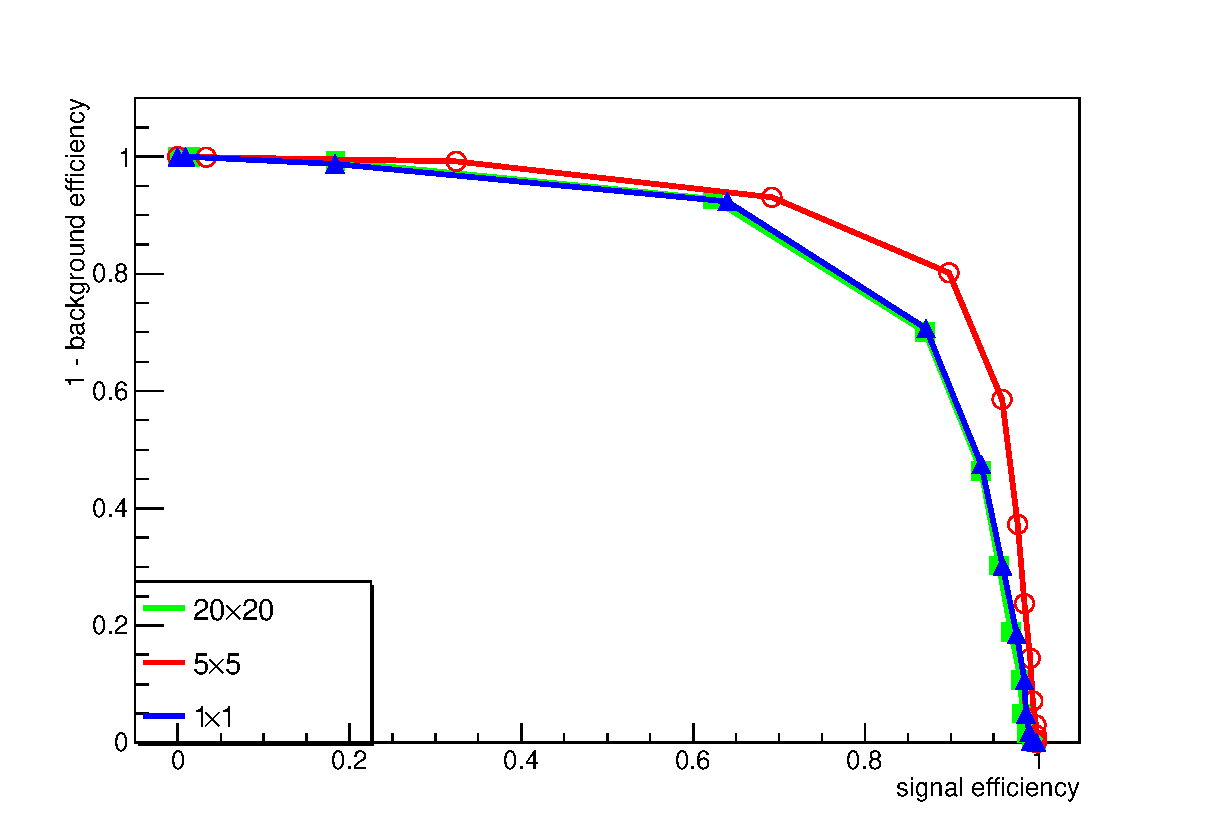
\includegraphics[width=0.43\textwidth]{figs/cluster_c2b1_40_tev_eff.eps}
   }
\end{center}
\caption{Signal efficiency versus background rejection rate using $c2b1$:We can see this variable is the best variable to separate the signal and background, because all lines are higher than other two variables (Figure 4 and Figure 5). But in the different size of separation efficiency in this variable, we can't see more improvement in, as you can see, all lines nearly merge together in all energy, it means all detector size has the similar separation efficiency.}
\label{fig:cluster_c2b1}
\end{figure}


\begin{figure}
\begin{center}
   \subfigure[5 TeV] {
   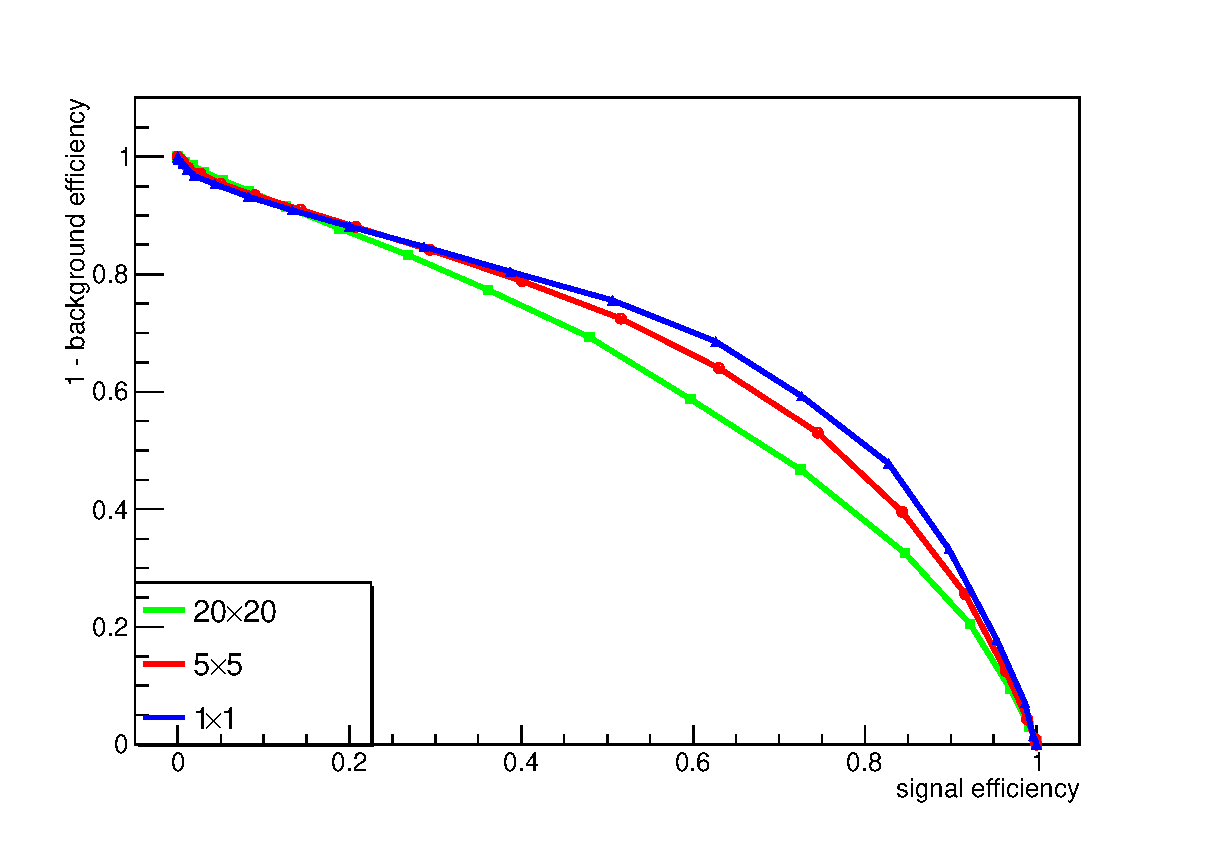
\includegraphics[width=0.43\textwidth]{figs/cluster_tau21_5_tev_eff.eps}\hfill
   }
   \subfigure[10 TeV] {
   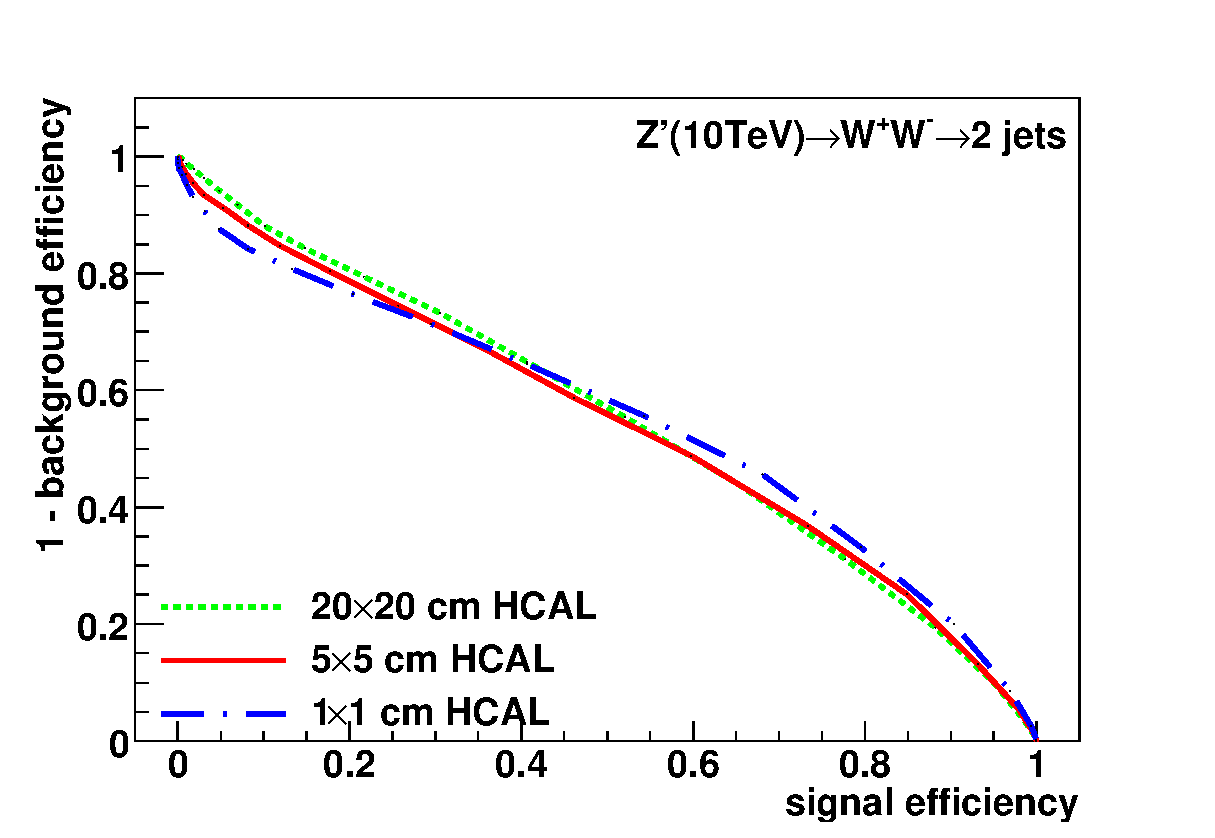
\includegraphics[width=0.43\textwidth]{figs/cluster_tau21_10_tev_eff.eps}
   }
   \subfigure[20 TeV] {
   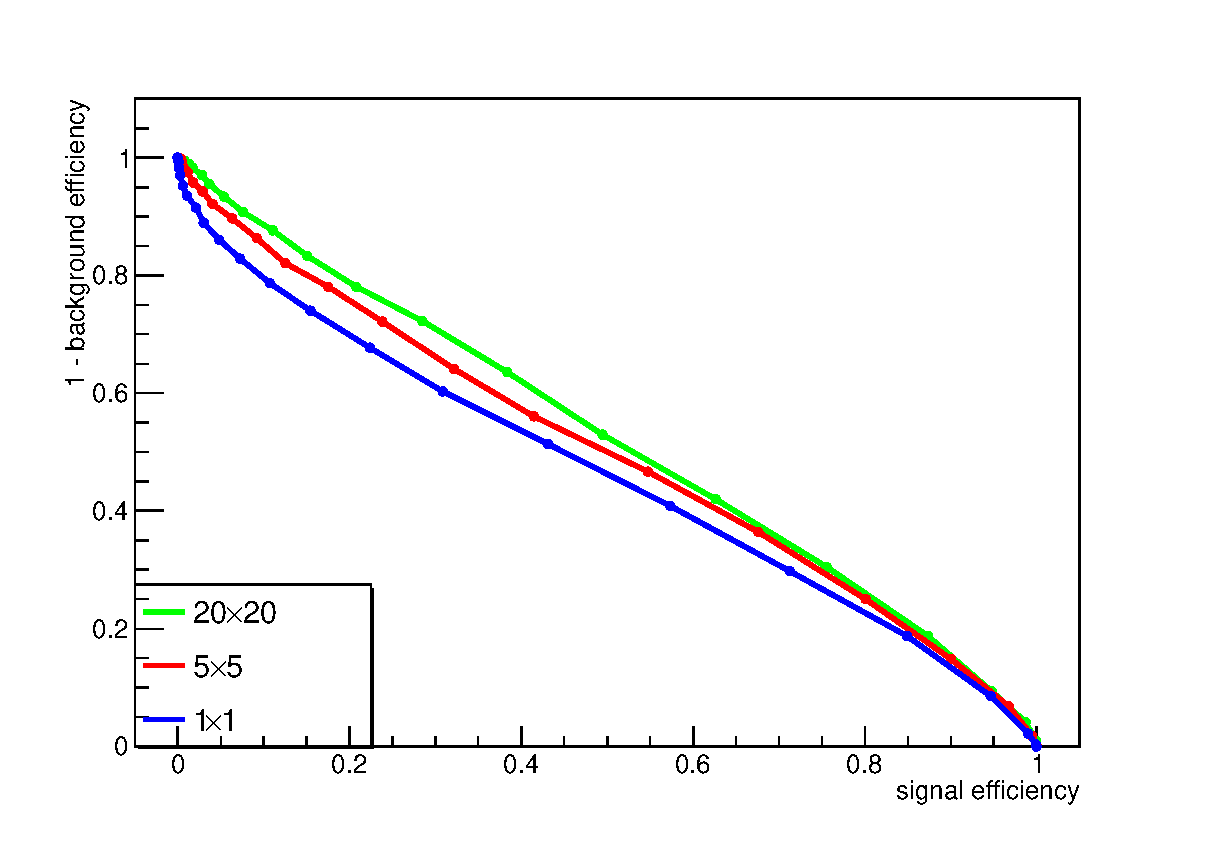
\includegraphics[width=0.43\textwidth]{figs/cluster_tau21_20_tev_eff.eps}
   }
   \subfigure[40 TeV] {
   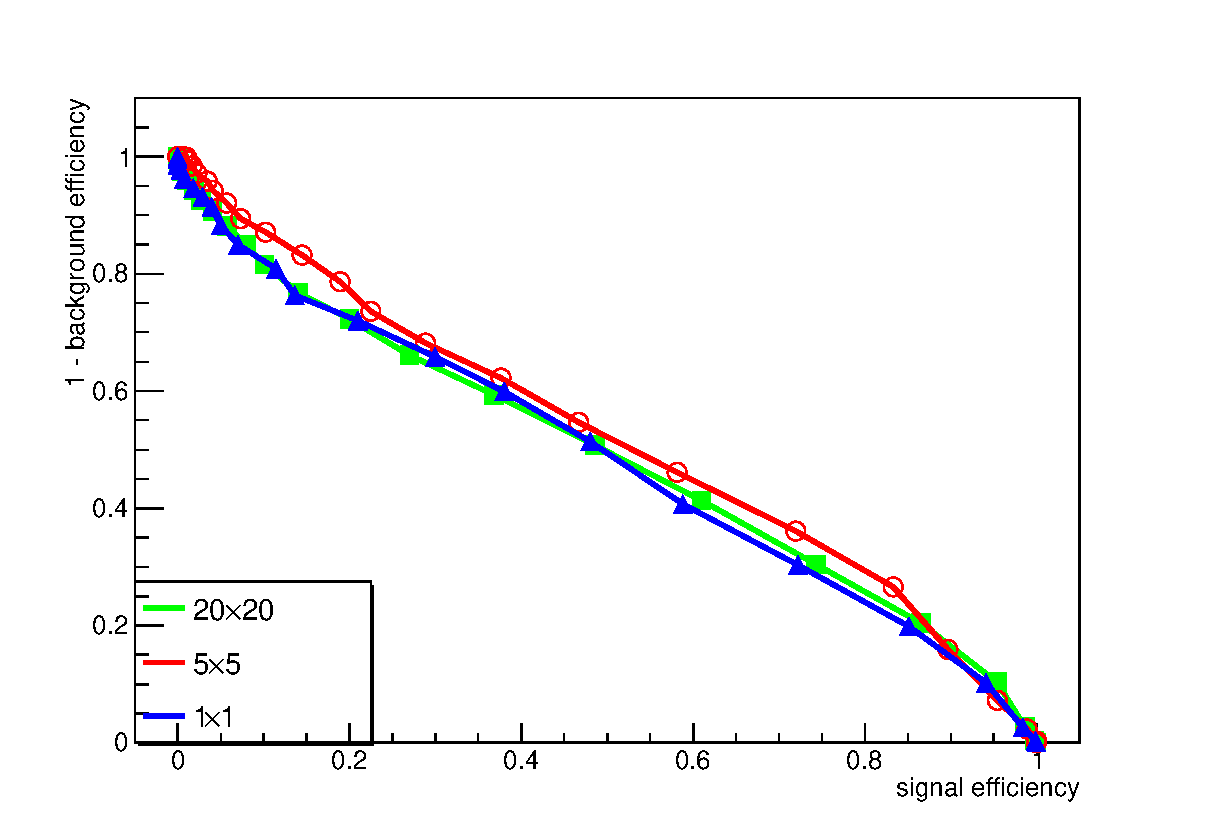
\includegraphics[width=0.43\textwidth]{figs/cluster_tau21_40_tev_eff.eps}
   }
\end{center}
\caption{Signal efficiency versus background rejection rate using $\tau_{21}$:we can see at 5 TeV in smallest detector size, it can separate signal and background well. But at 10TeV, all lines nearly merge together, they have similar separation efficiency. In 20TeV and 40TeV, we can see that it won't improve the separation efficiency. Specially, bigger detector size has the higher separation efficiency than smaller detector size.}
\label{fig:cluster_tau21}
\end{figure}


\begin{figure}
\begin{center}
   \subfigure[5 TeV] {
   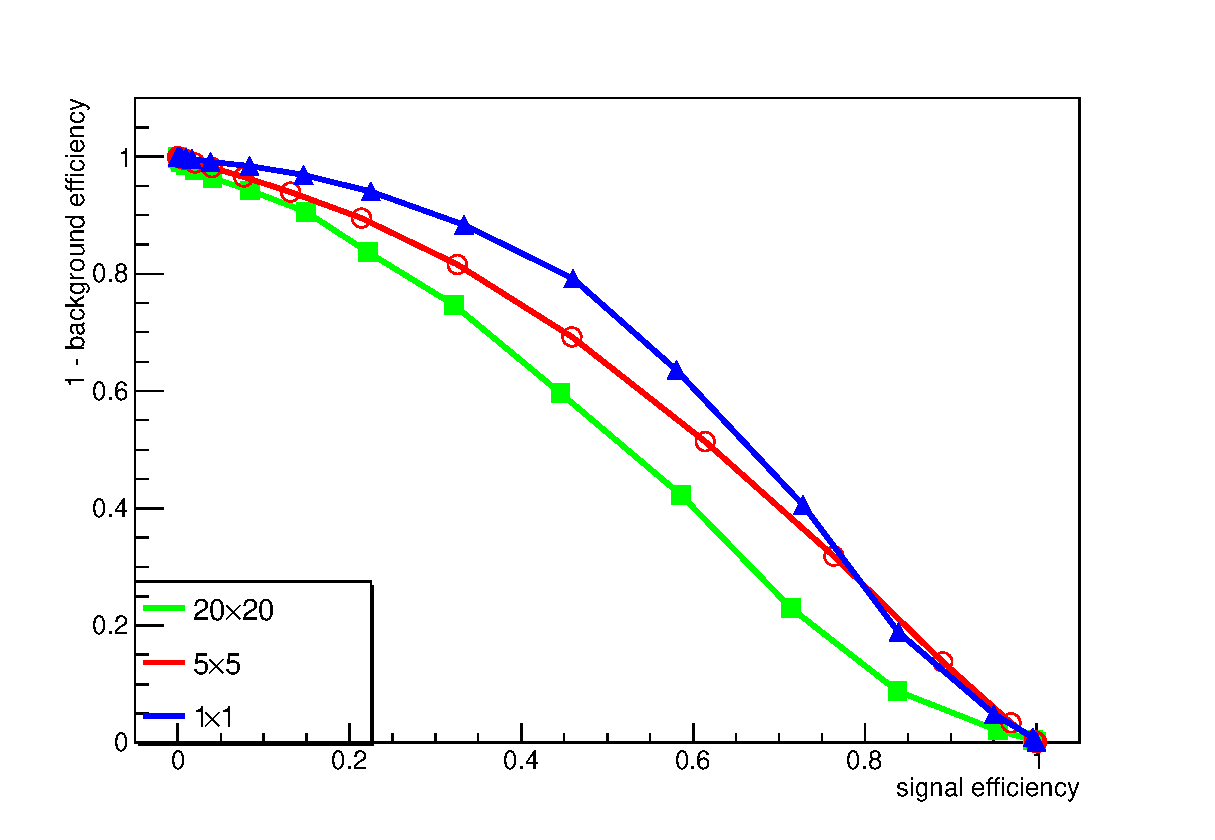
\includegraphics[width=0.43\textwidth]{figs/cluster_tau32_5_tev_eff.eps}\hfill
   }
   \subfigure[10 TeV] {
   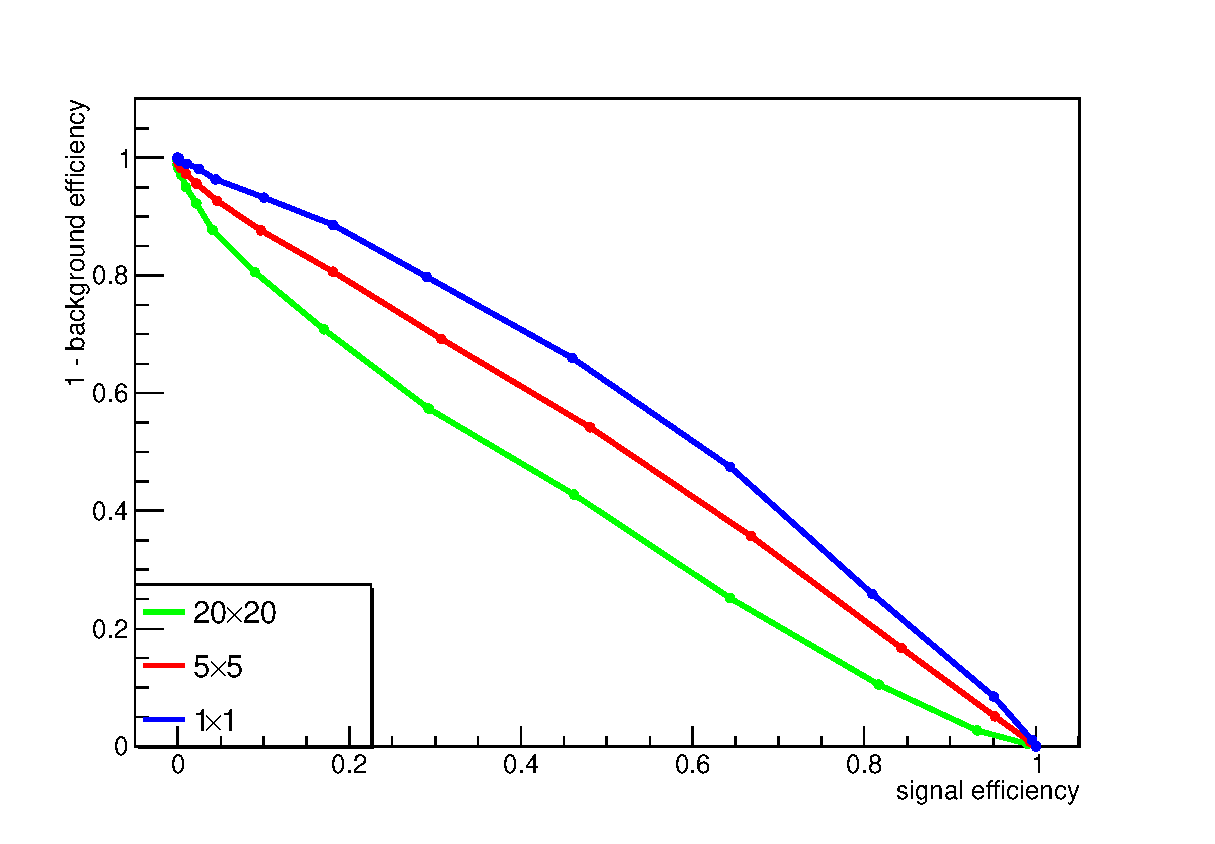
\includegraphics[width=0.43\textwidth]{figs/cluster_tau32_10_tev_eff.eps}
   }
   \subfigure[20 TeV] {
   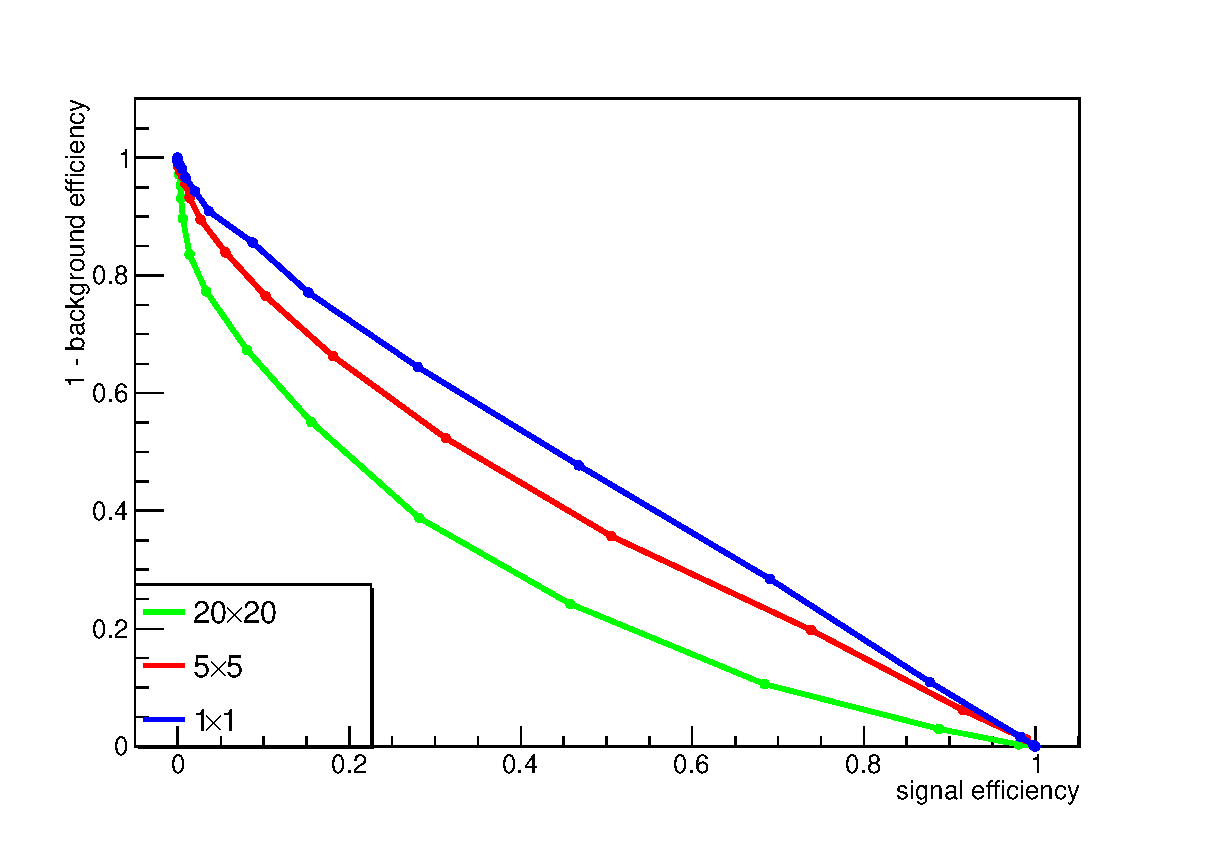
\includegraphics[width=0.43\textwidth]{figs/cluster_tau32_20_tev_eff.eps}
   }
   \subfigure[40 TeV] {
   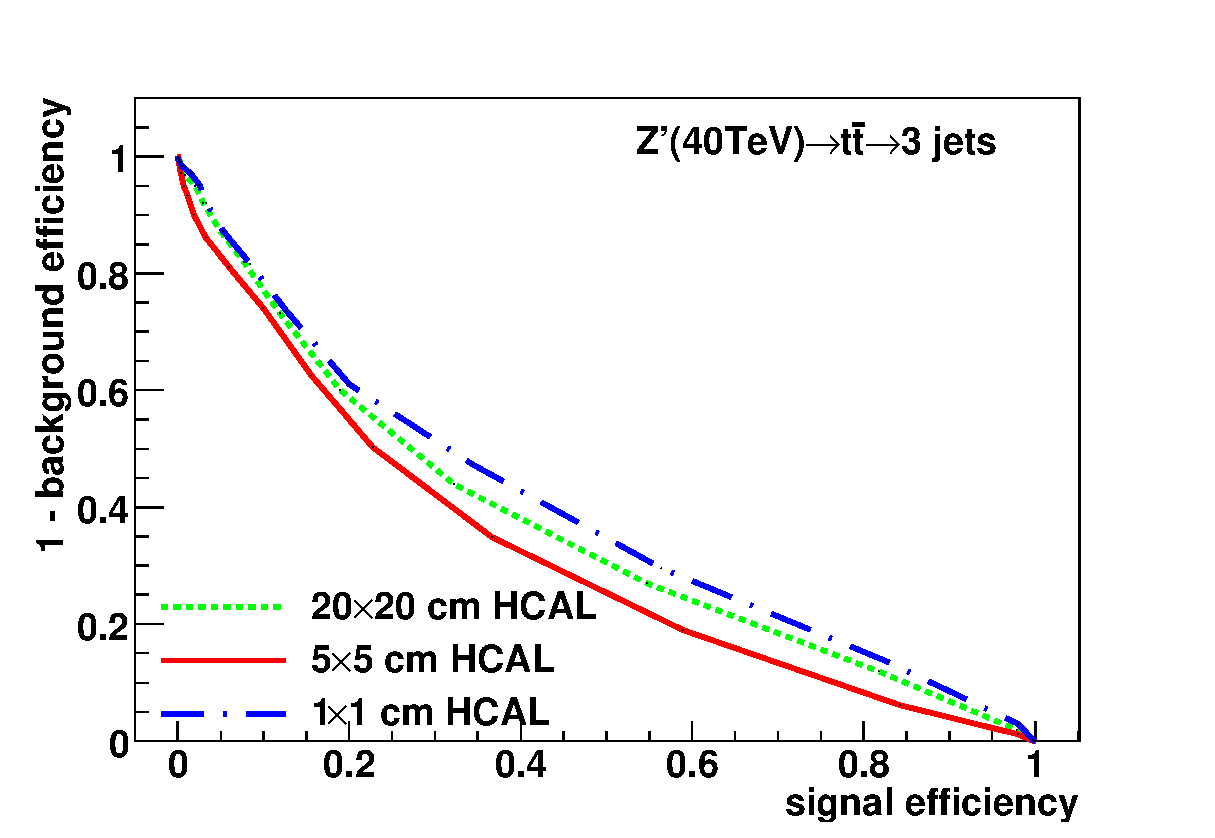
\includegraphics[width=0.43\textwidth]{figs/cluster_tau32_40_tev_eff.eps}
   }
\end{center}
\caption{Signal efficiency versus background rejection rate using $\tau_{32}$:we can see that it follows the role which smaller detector size have the bigger separation efficiency in all energy.}
\label{fig:cluster_tau32}
\end{figure}

